\documentclass[a4paper,12pt]{article}

\usepackage[utf8]{inputenc}
\usepackage[T1]{fontenc}
\usepackage[a4paper,total={150mm,240mm}]{geometry}



%%% packages %%%%%%%%%%%%%%%%%%%%%%%%%%%%%%%%%%%%%%%%%%%%%%%%%%%%%%%%%%%%%%%%%%
\usepackage[T1]{fontenc}        % euro quality fonts [T1] (togeth. w/ textcomp)
\usepackage{textcomp, amssymb}  % additional symbols (there are more packages)
\usepackage[utf8]{inputenc}   % umlaute in input file
\usepackage{setspace}           % doublespacing
\usepackage{anysize}            % margin package sets tighter margins
\usepackage[all]{xy}            % creating figures within latex

%\marginsize{1.2in}{0.9in}{1.1in}{0.9in} % small margins
\marginsize{1.2in}{0.9in}{0.5in}{1.5in} % small margins

%\usepackage[headings]{fullpage}
\usepackage{amsmath}
\usepackage{amsthm}
\usepackage{enumitem}
\usepackage{amsfonts}
\usepackage{graphicx}
\usepackage[first=0,last=9]{lcg}
\usepackage{multirow} %multirow in tables
\usepackage[margin=1cm]{caption} %special effects with floats captions
\usepackage{subcaption}
\usepackage{thumbpdf}
\usepackage{tikz} %to create pictures in tikz
\usepackage{siunitx, chemmacros} % chemical and SI units
%useful links in pdf
\usepackage[colorlinks,%
              pagebackref=false, % bibliography -> text
              linktocpage=true, % toc etc: make page number active (not name)
              plainpages=false, % distinguish roman and arabic pagenumbers
              bookmarksopen=true,%
              linkcolor=blue,
              bookmarksnumbered=true,%
              pdfauthor={Pavel Hron},%
              pdftitle={Phase Exchange in Porous Medium},%
              pdfsubject={report},%
              pdfkeywords={...},%
             ]{hyperref}        % clickabe references

% hyperref must be the second last package and glossary the last package
\usepackage{ctable}
\usepackage{listings}
\usepackage{afterpage}
\usepackage{tabularx}


%\usepackage{amsmath}
%\usepackage{amsfonts}
%\usepackage{amsthm}
%\usepackage{amscd}
%\usepackage{grffile}
%%some compile error
%%\usepackage{tikz}
%\usepackage{eurosym}
%\usepackage{graphicx}
%\usepackage{color}
%\usepackage{listings}
%\lstset{language=C++, basicstyle=\ttfamily,
%  keywordstyle=\color{black}\bfseries, tabsize=4, stringstyle=\ttfamily,
%  commentstyle=\itshape, extendedchars=true, escapeinside={/*@}{@*/}}
%\usepackage{paralist}
%\usepackage{curves}
%\usepackage{calc}
%\usepackage{picinpar}
%\usepackage{enumerate}
%\usepackage{algpseudocode}
%\usepackage{bm}
%\usepackage{multibib}
%\usepackage{hyperref}
%\usepackage{textcase}
%\usepackage{nicefrac}
%\usepackage{xspace} %spaces after some macros


\newcommand{\Seffalpha}{\gls{symb:effsatalpha}}

\newcommand{\Sl}{\mbox{$s_l\xspace$}}
\newcommand{\Slr}{\mbox{$s_{r,l}\xspace$}}
\newcommand{\Sgr}{\mbox{$s_{r,g}\xspace$}}
\newcommand{\Sle}{\mbox{$s_{e,l}\xspace$}}
\newcommand{\Sge}{\mbox{$s_{e,g}\xspace$}}
\newcommand{\Sls}{\mbox{$s_l^*\xspace$}}
\newcommand{\Sg}{\mbox{$s_g\xspace$}}
\newcommand{\dder}{\mbox{$\textrm{d}$}}

\newcommand{\agw}{\mbox{$a_{gw}\xspace$}}
\newcommand{\coxyw}{\mbox{$c_{l,O_2}\xspace$}}
\newcommand{\rp}{\mbox{$p_d\xspace$}} %mean particle diameter
\newcommand{\mo}{\mbox{$m_o\xspace$}}
\newcommand{\vl}{\mbox{$\bf{v}_{l}\xspace$}}
\newcommand{\kl}{\mbox{$k_L\,\alpha\xspace$}}

\newcommand{\cnp}{\mbox{$c_{np}\xspace$}}
\newcommand{\cnpi}{\mbox{$c_{np,0}\xspace$}}
\newcommand{\snp}{\mbox{$S_{np}\xspace$}}
\newcommand{\snpe}{\mbox{$S_{np}^e\xspace$}}
\newcommand{\npinit}{\mbox{$C_0\xspace$}}
\newcommand{\snpmax}{\mbox{$S_{np,max}\xspace$}}
\newcommand{\coxyg}{\mbox{$c_{g,O_2}\xspace$}}
\newcommand{\coxys}{\mbox{$c^*_{l,O_2}\xspace$}}



\newcommand{\coxysg}{\mbox{$c^*_{g,O_2}\xspace$}}

\newcommand{\kh}{\mbox{$k_H\xspace$}}
\newcommand{\khcc}{\mbox{$k_{H}^{cc}\xspace$}}
\newcommand{\pgk}{\mbox{$p_{g,k}$}}
\newcommand{\cak}{\mbox{$c^*_{l,k}$}}
\newcommand{\cake}{\mbox{$c_{l,k}$}}
\newcommand{\cgke}{\mbox{$c_{g,k}$}}




\title{Static and dynamic phase mass transfer models of gases with a
  low solubility applicatable in porous media}
\author{Pavel Hron}
\date{\today}

\begin{document}
\maketitle

\subsubsection*{Dynamic Model of Oxygen Transfer}
Many chemical and biological processes, e.g. dissolved iron oxidation
or aerobic microbiological growth in porous medium, are dependent on
the supply of oxygen to the liquid phase.

To specify the macro-scale closure relationships for the mass transfer
of oxygen between gas and water phase in porous media, we follow the
model discussed in \cite{Geistlinger2005} and \cite{Holocher2003}
based on the stagnant film model for a spherical gas bubbles. Many
mass transfer theories implicitly assumes that the rate of inter-phase
transfer is a function of a driving force and an interfacial area
between phases. If we assume that the activities can be approximated
by the concentrations, the mass transfer for oxygen in water and in
air is given by
\begin{equation} - e_{g,O_2} = e_{l,O_2}=\beta \agw \left(\coxys -
\coxyw \right),
\end{equation} where $\beta$ is the mass transfer coefficient, $\agw$
is the effective gas-water interface, $\coxys$ is dissolved oxygen
concentration at equilibrium and $\coxyw$, $\coxyg$ correspond to the
dissolved oxygen concentration in water and gas phase, respectively.

Dynamic mass balance equations for oxygen in the liquid and in the gas
phase can be written as
\begin{align} \frac{\dder \left(\phi \Sl \coxyw \right)}{\dder \, t}
&= e_{l,O_2}, \label{Eq:OxygenTransfera} \\ \frac{\dder \left(\phi \Sg
\coxyg \right)}{\dder \, t} &= e_{g,O_2}, \label{Eq:OxygenTransferb}
\end{align} where $\phi$ is porosity, $\Sl$ and $\Sg$ are liquid and
gas saturation.

\subsubsection*{Henry's Law}

Mass transfer between liquid and gas phase occurs at the phase
interface. For gases with a low solubility, like oxygen in water, the
solubility of a gas in a liquid phase is directly proportional to the
partial pressure of the gas above the liquid
\begin{equation} \pgk \kh = \cake, \label{Eq:HenryLaw}
\end{equation} where $\pgk$ is the partial pressure of the solute in
the gas phase, $\kh$ is the Henry's law constant and $\cak$ is the
equilibrium molar concentration in the liquid phase. Introducing a
dimensionless constant $\khcc=\kh \cdot RT$, Henry's law
\eqref{Eq:HenryLaw} is given by \cite{Sander1999}
\begin{equation} \cake = \khcc \cgke.  \label{Eq:HenryLaw2}
\end{equation} The Henry's law constant generally depends on the
solute, the solvent, the pressure and the temperature.

\subsubsection*{Static Model of Oxygen Transfer}
If the dissolution of oxygen is fast enough, we can omit the dynamic
effect of the mass transfer. The dissolved oxygen concentration at equilibrium
with the gas phase is expressed from Henry's law \eqref{Eq:HenryLaw}
as
\begin{equation} \label{Eq:OxygenEquilibrium} \coxys = \kh \, \coxyg
\,R \,T = \khcc \, \coxyg .
\end{equation}
While in the porous medium the total amount of oxygen depends on water
and gas saturation, the total oxygen mass should stay constant:
\begin{equation}\label{Eq:OxygenMassConservation}
  \begin{pmatrix}
    \Sl & \Sg \\
    1 & -\khcc\\
  \end{pmatrix}
  \begin{pmatrix}
    \coxys \\
    \coxysg \\
  \end{pmatrix}
  =
  \begin{pmatrix}
    \Sl & \Sg \\
    0 & 0\\
  \end{pmatrix}
  \begin{pmatrix}
    \coxyw \\
    \coxyg  \\
  \end{pmatrix}
\end{equation}
From equation \eqref{Eq:OxygenMassConservation} we can express oxygen
concentration for both phases in equilibrium ($\coxys, \coxysg$) as
\begin{equation}\label{Eq:OxygenMassConservationResult}
  \begin{pmatrix}
    \coxys \\
    \coxysg \\
  \end{pmatrix}
  =
  \frac{1}{\Sl \khcc + \Sg}
  \begin{pmatrix}
    \khcc  & \Sg \\
    1 & -\Sl\\
  \end{pmatrix}
  \begin{pmatrix}
    \Sl & \Sg \\
    0 & 0\\
  \end{pmatrix}
  \begin{pmatrix}
    \coxyw \\
    \coxyg  \\
  \end{pmatrix}
  =
  \frac{1}{\Sl \khcc + \Sg}
  \begin{pmatrix}
    \khcc \Sl  & \khcc \Sg \\
    \Sl & \Sg\\
  \end{pmatrix}
  \begin{pmatrix}
    \coxyw \\
    \coxyg  \\
  \end{pmatrix}
\end{equation}


\subsubsection*{Mass transfer coefficient}
The mass transfer coefficient $\beta$ for a spherical structure with
the harmonic mean particle diameter $\rp$ is given by \cite{Clift1978}
\begin{equation} \beta =
\frac{D_{l,O_2}}{\delta_{eff}}=D_{l,O_2}\left(\frac{2}{\rp}+\frac{1}{\delta}\right),\label{Eq:masstransfercoeff}
\end{equation} where $D_{l,O_2}$ is the oxygen diffusion coefficient
in water and $\delta$ is the thickness of the stagnant film layer.

For advection flow regimes, the boundary layer thickness depends on
the interface velocity $\vl$. The difference between flow and
interface velocity directly at the interface is in most cases very
small and therefore neglected \cite{Niessner2011}. In this case, the
thickness of the film layer can be expressed by \cite{Holocher2003}
\begin{equation*} \delta=\sqrt{\frac{\pi \rp D_{l,O_2}}{\vl}}.
\end{equation*} Comparison of different mass transfer
coefficient-velocity correlations for oxygen can be found in
\cite{Geistlinger2005}.

\subsection*{Gas-liquid inter-facial area}

The gas-liquid interface
plays a crucial role in the mass transfer in unsaturated porous
media. Constitutive relationships between gas-liquid specific
inter-facial area, capillary pressure and saturation have already been
derived either from pore-scale network models \cite{Cary1994,
Niemet2002, Anwar2008, Gvirtzman1991, Reeves1996, Joekar-Niasar2007,
Held2001}, from Lattice-Boltzmann simulations \cite{Ahrenholz2011} or
from experiments \cite{Brusseau1997, Chen2006, Culligan2004,
FaisalAnwar2000, Kim1999, Schaefer2000, Porter2010}.

Some proposed models are expecting the maximum degree of gas-liquid
inter-facial area available for a particular porous medium occurs near
to residual liquid saturation \cite{Cary1994, Niemet2002,
Gvirtzman1991, Anwar2008}. However, the network models
\cite{Reeves1996, Held2001, Joekar-Niasar2007} show that gas-liquid
inter-facial area increases linearly with decreasing water saturation
until a limit water saturation $\Sls$ is reached and then the
inter-facial area rapidly decreases until the area reaches zero as the
water saturation approaches zero.

The experimental techniques used to measure inter-facial area
\cite{Chen2006, FaisalAnwar2000, Kim1999, Schaefer2000}, have all
found monotonic increase in inter-facial area as $\Sl \rightarrow 0$
(with decreasing saturation), but results of experiments with glass
beads in \cite{Culligan2004, Porter2010} showed a good agreement with
the pore network modeling \cite{Reeves1996}. This does not indicate
that any one of these experimental methods is necessarily
wrong. Rather, there is a lack of understanding concerning which
interfaces are being detected in any of these experimental
techniques. However, in both types of studies, the gas-liquid
interface is roughly proportional to the gas content $\Sg$ for
$\Sl>\Sls$, where $\Sls=0.2-0.3$, which covers the main region of our
interest.

As was pointed out in \cite{Porter2010}, there are differences in
predicting liquid-gas inter-facial area for drainage and imbibition
experiments, but the behavior of both processes is similar
\cite{Culligan2004}. A comparison between experimental total
inter-facial area curves for solid surface area and water-air
inter-facial area can be found in \cite{Porter2010}.

A basic model based on geometrically relationships to estimate the
total surface area for any packing of spheres was presented by
\cite{Gvirtzman1991}. The total effective interstitial particle
surface area per unit bulk volume is given by
\begin{equation} \agw =\kappa \Sg
\frac{6(1-\phi)}{\rp}, \label{Eq:surfaceAreaGvirtzman1991}
\end{equation} where $\kappa$ is the fraction of air bubble surface
area exposed to mobile water. This empirical factor is often
approximated by the porosity \cite{Geistlinger2005}. Similar model to
\eqref{Eq:surfaceAreaGvirtzman1991} was used in
\cite{Geistlinger2005}:
\begin{equation} \agw = \kappa \Sg
\frac{6\phi}{\rp}, \label{Eq:surfaceAreaBasic}
\end{equation}


% \cite{Culligan2004}:
% experiment surface (up to $\Sl = 0.3$ linear, maximal surface are
% $a=\SI{0.25}{\per \milli \meter}$, good comparison with
% \cite{Reeves1996}

% \cite{Schaefer2000}
% However, scatter in the data due to
% experimental difficulty in measuring the interfacial area at very low
% $(\Sl < 0.08)$ water saturations made this diffiult.
% maximal area is $a=\SI{0.2}{\per \milli \meter}$
% the air-water interfacial area decreased almost linearly with
% saturation, while imbibition experiments showed a more complex
% nonmonotonic relation to the saturation

More sophisticated approach to determine the gas-liquid inter-facial
area derived from a distribution of spherical pores was proposed by
\cite{Niemet2002}. Under the assumption that the pores are discrete
and symmetrical in all dimensions, following equation to determine
effective gas-liquid surface area was derived
\begin{equation}
  \agw = \frac{3\phi}{2\sigma}
  \int_{0}^{\Sl}p_c(S) \, dS, \label{Eq:surfaceAreaNiemet}
\end{equation}
where $\sigma$ is the surface tension of the liquid. In contrast to
model \eqref{Eq:surfaceAreaGvirtzman1991}, that depends only on
porosity $\phi$, model \eqref{Eq:surfaceAreaNiemet} takes into account
the pore distribution.

For a van Genuchten parametrization \cite{Genuchten1980},
the integral in \eqref{Eq:surfaceAreaNiemet} can be computed
analytically using the substitution $z=1+\frac{1}{n}$, $w=m-1/n$,
where $n,m$ are parameters in van Genuchten model (see
\cite{Niemet2002}, eq. (15). Equation \eqref{Eq:surfaceAreaNiemet} can
be expressed as
\begin{equation} \agw = \Sg %
  \frac{3\phi}{2\sigma} \frac{m}{\alpha}
  B(w,z)\left(1-I_u(w,z)\right), \label{Eq:surfaceAreaNiemetComputed}
\end{equation}
where $B(w,z)$ is the beta function and $I_u(w,z)$
represents the incomplete beta function.

The comparison of different models with model based on fitting a bi-quadratic
polynomial to the experimental data as in \cite{Porter2010} are in
Fig. \ref{fig:interfacial_area}.
\begin{figure*}
  \centering
  \resizebox{0.95\linewidth}{!}{\begin{picture}(0,0)%
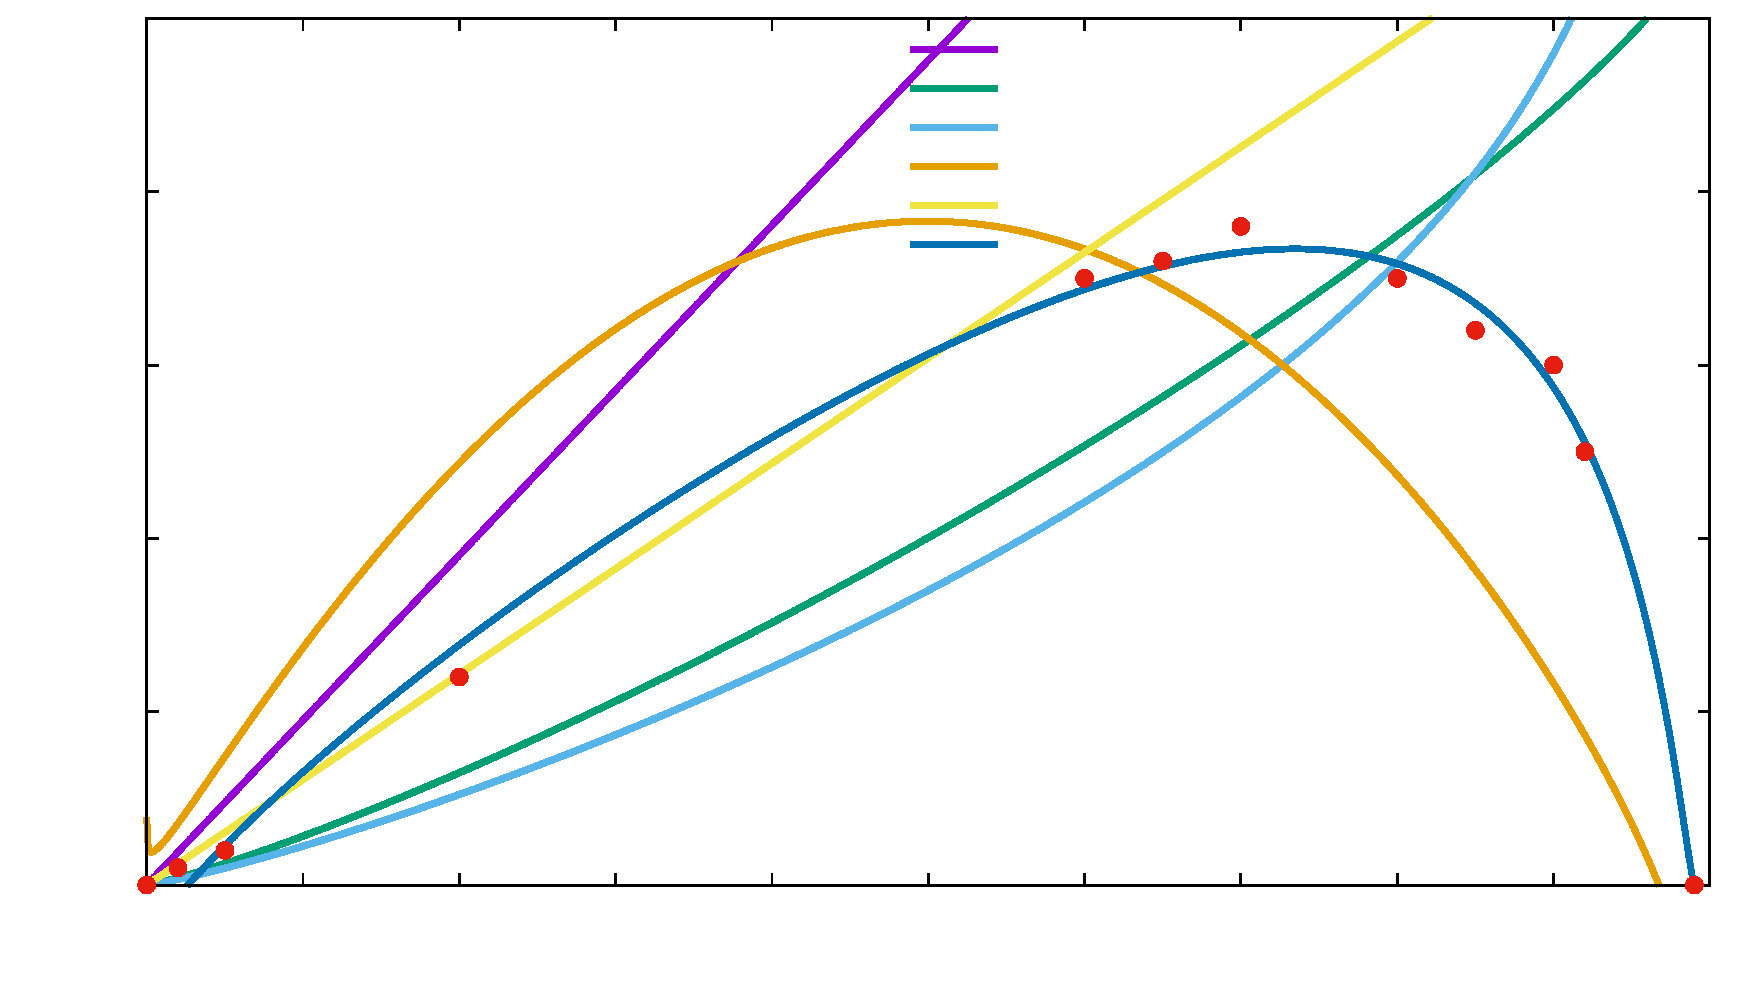
\includegraphics{./interfacial_area}%
\end{picture}%
\setlength{\unitlength}{4144sp}%
%
\begingroup\makeatletter\ifx\SetFigFont\undefined%
\gdef\SetFigFont#1#2{%
  \fontsize{#1}{#2pt}%
  \selectfont}%
\fi\endgroup%
\begin{picture}(13263,7538)(944,-7750)
%  Begin plot #1 
\put(7742,-703){\makebox(0,0)[rb]{\smash{{\SetFigFont{20}{24.0}model by \cite{Gvirtzman1991}, eq \eqref{Eq:surfaceAreaGvirtzman1991}}}}}
%  Begin plot #2 
\put(7742,-1000){\makebox(0,0)[rb]{\smash{{\SetFigFont{20}{24.0}model by \cite{Niemet2002}, eq \eqref{Eq:surfaceAreaNiemetComputed}}}}}
%  Begin plot #3 
\put(7742,-1297){\makebox(0,0)[rb]{\smash{{\SetFigFont{20}{24.0}model by \cite{Miller1990}}}}}
%  Begin plot #4 
\put(7742,-1594){\makebox(0,0)[rb]{\smash{{\SetFigFont{20}{24.0}model by \cite{Joekar-Niasar2007} based on data \cite{Culligan2004}}}}}
%  Begin plot #5 
\put(7742,-1891){\makebox(0,0)[rb]{\smash{{\SetFigFont{20}{24.0}model by \cite{Geistlinger2005}}}}}
\put(1920,-7069){\makebox(0,0)[rb]{\smash{{\SetFigFont{20}{24.0} 0}}}}
\put(1920,-5748){\makebox(0,0)[rb]{\smash{{\SetFigFont{20}{24.0} 100}}}}
\put(1920,-4427){\makebox(0,0)[rb]{\smash{{\SetFigFont{20}{24.0} 200}}}}
\put(1920,-3107){\makebox(0,0)[rb]{\smash{{\SetFigFont{20}{24.0} 300}}}}
\put(1920,-1786){\makebox(0,0)[rb]{\smash{{\SetFigFont{20}{24.0} 400}}}}
\put(1920,-465){\makebox(0,0)[rb]{\smash{{\SetFigFont{20}{24.0} 500}}}}
\put(13974,-7307){\makebox(0,0)[b]{\smash{{\SetFigFont{20}{24.0}0.0}}}}
\put(12783,-7307){\makebox(0,0)[b]{\smash{{\SetFigFont{20}{24.0}0.1}}}}
\put(11592,-7307){\makebox(0,0)[b]{\smash{{\SetFigFont{20}{24.0}0.2}}}}
\put(10400,-7307){\makebox(0,0)[b]{\smash{{\SetFigFont{20}{24.0}0.3}}}}
\put(9209,-7307){\makebox(0,0)[b]{\smash{{\SetFigFont{20}{24.0}0.4}}}}
\put(8018,-7307){\makebox(0,0)[b]{\smash{{\SetFigFont{20}{24.0}0.5}}}}
\put(6827,-7307){\makebox(0,0)[b]{\smash{{\SetFigFont{20}{24.0}0.6}}}}
\put(5636,-7307){\makebox(0,0)[b]{\smash{{\SetFigFont{20}{24.0}0.7}}}}
\put(4444,-7307){\makebox(0,0)[b]{\smash{{\SetFigFont{20}{24.0}0.8}}}}
\put(3253,-7307){\makebox(0,0)[b]{\smash{{\SetFigFont{20}{24.0}0.9}}}}
\put(2062,-7307){\makebox(0,0)[b]{\smash{{\SetFigFont{20}{24.0}1.0}}}}
\put(1150,-3648){\rotatebox{-270.0}{\makebox(0,0)[b]{\smash{{\SetFigFont{20}{24.0}interfacial area  [\si{\per \meter}]}}}}}
\put(8018,-7664){\makebox(0,0)[b]{\smash{{\SetFigFont{20}{24.0}water saturation [-]}}}}
\end{picture}%
}
  \caption{Water-gas inter-facial area computed with different
    models. Used parameters: $\phi=0.39$, $\alpha=0.0012$, $n=5.48$, $\rp=1.5e-3\text{m}$.}
  \label{fig:interfacial_area}
\end{figure*}

% bibtex bibliography
\bibliographystyle{abstract}
\bibliography{references.bib}

\end{document}
